\subsubsection{HVAE for Efficient Generation of Mathematical Expressions}

In \emph{Efficient Generator of Mathematical Expressions for Symbolic
Regression}, \citet{meznar2023efficient} address the generation of candidate
equations for symbolic regression. Their central model is a hierarchical
variational autoencoder (HVAE) that represents every expression directly as a
binary tree: internal nodes contain binary operators or unary functions, while
leaves contain variables or constants. The associated EDHiE method searches
the HVAE's continuous latent space for an expression whose evaluated values
fit an observed dataset. This makes the paper relevant to the formula-sampling
stage of the proposed benchmark: a learned prior over trees can concentrate
samples around expression structures found in a selected scientific domain.

\paragraph{Where the training trees come from.}
Before HVAE can sample new expressions, it learns from a corpus of valid trees.
In the experiments, this corpus is produced with probabilistic context-free
grammars and then simplified with SymPy. One reported arithmetic grammar
recursively selects addition or subtraction, multiplication or division, and
parenthesized subexpressions, constants, or variables; a second version also
contains sine and cosine. Consequently, HVAE learns the distribution supplied
by its training corpus rather than beginning from an empty expression space.
For the present thesis, that corpus could instead contain safe discrete-time
mechanisms whose leaves are constants, the current index, and
$\operatorname{LAG}(j,\ell)$ terms.

\paragraph{How HVAE learns a distribution over trees.}
The encoder processes a tree bottom-up. At node $v$, a GRU$_{2\rightarrow1}$
cell combines the symbol stored at $v$ with the representations of its left and
right children. The final root representation is mapped to the mean and
log-variance of a Gaussian latent code. The decoder reverses this direction.
It maps a latent vector to a root state and recursively expands the tree with a
GRU$_{1\rightarrow2}$ cell whose shared parameters are reused at every node.
In the notation of this review, one decoding step is

\begin{equation}
\begin{aligned}
\mathbf z &\sim \mathcal N(\mathbf 0,\mathbf I),
&\mathbf h_{\varnothing}&=\mathbf W_z\mathbf z+\mathbf b_z,\\
\boldsymbol\pi_v
  &=\operatorname{softmax}(\mathbf W_s\mathbf h_v+\mathbf b_s),
&s_v&=\arg\max_s \pi_{v,s},\\
(\mathbf h_{vL},\mathbf h_{vR})
  &=\operatorname{GRU}_{1\rightarrow2}
    (\boldsymbol\pi_v,\mathbf h_v).&&
\end{aligned}
\label{eq:meznar-hvae-decoder}
\end{equation}

The selected symbol determines the tree structure. A binary operator activates
both child states, a unary function activates only the left child, and a
variable or constant terminates that branch. The released decoder selects the
largest softmax probability and, at the configured maximum height, restricts
the choice to leaf symbols.\footnote{Official HVAE implementation:
\url{https://github.com/smeznar/HVAE}; see the recursive decoding and
\texttt{sample\_symbol} routines in \texttt{EDHiE/model.py}.} Thus a latent
draw leads to a complete tree by the following recursion:

\begin{enumerate}
    \item sample $\mathbf z\sim\mathcal N(\mathbf 0,\mathbf I)$ and transform it
    into the root state $\mathbf h_{\varnothing}$;
    \item calculate $\boldsymbol\pi_v$ and choose symbol $s_v$ at the current
    node;
    \item if $a(s_v)=2$, create and decode the left and right child states;
    if $a(s_v)=1$, decode only the left state; if $a(s_v)=0$, close the branch;
    \item repeat the same decoder cell until every branch reaches a leaf;
    \item fit any free constants and execute the resulting expression when it
    is evaluated as a symbolic-regression candidate.
\end{enumerate}

\begin{figure}[H]
\centering
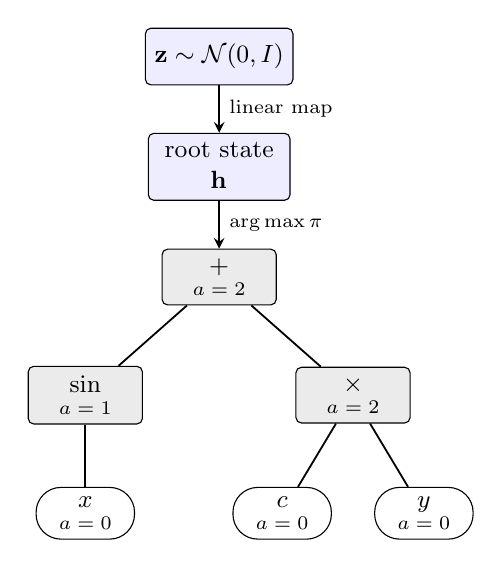
\begin{tikzpicture}[
    state/.style={
        draw,
        rounded corners=2pt,
        fill=blue!7,
        minimum width=1.8cm,
        minimum height=0.72cm,
        align=center,
        font=\small
    },
    operator/.style={
        draw,
        rounded corners=2pt,
        fill=black!8,
        minimum width=1.45cm,
        minimum height=0.68cm,
        align=center,
        font=\small
    },
    leaf/.style={
        draw,
        rounded corners=9pt,
        fill=white,
        minimum width=1.25cm,
        minimum height=0.62cm,
        align=center,
        font=\small
    },
    flow/.style={->,>=stealth,draw,line width=0.7pt},
    branch/.style={draw,line width=0.65pt}
]
    \node[state] (latent) at (0,1.8)
        {$\mathbf z\sim\mathcal N(0,I)$};
    \node[state] (rootstate) at (0,0.4)
        {root state\\$\mathbf h_{\varnothing}$};
    \node[operator] (add) at (0,-1.0)
        {$+$\\[-1mm]{\scriptsize $a=2$}};
    \node[operator] (sin) at (-1.7,-2.5)
        {$\sin$\\[-1mm]{\scriptsize $a=1$}};
    \node[operator] (mul) at (1.7,-2.5)
        {$\times$\\[-1mm]{\scriptsize $a=2$}};
    \node[leaf] (x) at (-1.7,-4.0)
        {$x$\\[-1mm]{\scriptsize $a=0$}};
    \node[leaf] (c) at (0.8,-4.0)
        {$c$\\[-1mm]{\scriptsize $a=0$}};
    \node[leaf] (y) at (2.6,-4.0)
        {$y$\\[-1mm]{\scriptsize $a=0$}};

    \draw[flow] (latent) -- node[right,font=\scriptsize]{linear map}
        (rootstate);
    \draw[flow] (rootstate) -- node[right,font=\scriptsize]{$\arg\max\boldsymbol\pi$}
        (add);
    \draw[branch] (add) -- (sin);
    \draw[branch] (add) -- (mul);
    \draw[branch] (sin) -- (x);
    \draw[branch] (mul) -- (c);
    \draw[branch] (mul) -- (y);
\end{tikzpicture}
\caption{Top-down HVAE decoding of one latent draw into the valid expression
$\sin(x)+c\,y$. Each predicted symbol determines how many descendant states
are decoded: two for a binary operator, one for a unary function, and zero for
a leaf.}
\label{fig:meznar-hvae-sampling}
\end{figure}

The standard sampling method, HVAR, repeats this process for independent
Gaussian latent draws. EDHiE searches the same space more deliberately: its
initial population is sampled from $\mathcal N(\mathbf 0,\mathbf I)$, crossover
forms convex combinations of two parent vectors, and mutation interpolates
between the encoded neighborhood of one expression and the standard Gaussian
prior. Candidate fitness is calculated only after decoding the vector, fitting
its constants, and evaluating the resulting equation on the observations
\citep{meznar2023efficient}.

\paragraph{Efficiency and relevance to the benchmark.}
The experiments report syntactically valid HVAE outputs, substantially lower
reconstruction error with 2,000 training expressions than the sequential VAE
obtains with 12,000, and effective operation in a 32-dimensional latent space.
On the Nguyen benchmark, latent-space random search reconstructs more equations
than the manually specified probabilistic-grammar baseline, while EDHiE adds an
evolutionary search over the learned space. For the proposed benchmark, HVAE
could therefore replace uniform formula sampling with a domain-shaped prior.
Its symbol library would include $\operatorname{LAG}(j,\ell)$, and each decoded
tree would pass numerical-domain, stability, variable-coverage, and recurrence
checks before it generated a time series. The retained decoded tree would then
supply the same structural, coefficient, local-contribution, gradient, and
Shapley references defined elsewhere in this thesis.

